\documentclass[10pt,a4paper]{report}

\usepackage[utf8]{inputenc}
\usepackage{amsmath}
\usepackage{amsfonts}
\usepackage{amssymb}
\usepackage{graphicx}
\usepackage{hyperref}
\usepackage[left=2cm,right=2cm,top=2cm,bottom=2cm]{geometry}

\title{Product Vision and Planning}
\author{Programming Life group 2\\
	\begin{tabular}{c c c}
	\hline 
		Derk-Jan Karrenbeld & 4021967 & 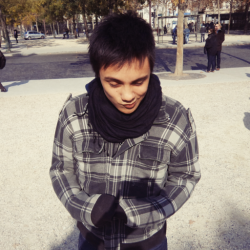
\includegraphics[scale=0.2]{../img/DJ.png}\\ 
		Joost Verdoorn & 1545396 & 
\includegraphics[scale=0.2]{../img/Yoloost.png}\\ 
		Steffan Sluis & 4088816 & 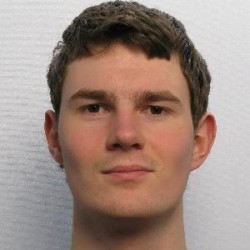
\includegraphics[scale=0.2]{../img/SS.jpeg}\\ 
		Tung Phan & 4004868 & 
\includegraphics[scale=0.2]{../img/TP.jpeg}\\ 
		Vincent Robbemond & 4174097 & 
\includegraphics[scale=0.2]{../img/VR.jpeg}\\ 
		\hline 
	\end{tabular} 
}
\date{\today}

\begin{document}
	\maketitle

	\section*{Preface}
		This document is a draft for the product vision and planning for the Context Project `Programming Life: Synthetic Biology'. It’s a proposition for the project structure, workflow and product target result that we will engage in and with during the period of the course. It contains a schedule with set dates, milestones and goals to be achieved and is a guideline for the work that should be done. The contents of this document are subject to changes and should be regarded as such.

	\setcounter{section}{0}
	\setcounter{secnumdepth}{3}
	\setcounter{tocdepth}{5}
	\renewcommand*\thesection{\arabic{section}}
	
	\pdfbookmark{\contentsname}{toc}
	\tableofcontents

	\clearpage

	\section{Introduction}
		Synthetic biologists try to create cells that work in certain ways. Before they accomplish this, they would like to simulate the internal workings of cells and their outputs by using combinations of several differential equations which influence each other. 
By varying the properties, say factors and values used by these equations, the biologists can simulate the output of the cell and measure the effect of that set of factors. 
However, the complexity of the simulation can be daunting if done on paper or programmed by hand per set of factors which is also time-consuming.\\

GigaBase is an intuitive application that should overcome this last problem by providing a GUI and allow the simulation of an extensive number of modules with user-specified properties and environment and thereby simulate a complete cell.
A module simulates a part of a cell by solving a systems of ODE describing its behaviour. 

By using this application, the user can efficiently find the optimal properties with less work to get their preferred outcome, such as maximizing the product of a cell. The user also doesn't have to worry about doing calculations which are prone to error and take a long time to perform.
\\

This product will be developed using the Scrum methodologies and the development wil be iterated in weekly sprints.

	\clearpage

	\section{Product}
		This section holds the main product vision, the high level product backlog and a general roadmap for the contents of the product in the duration of the project.
		\subsection{Product Vision}

			\textbf{FOR} Synthetic Biologists \textbf{WHO LIKE TO} create cells that work in certain ways, GigaBase \textbf{IS AN} application \textbf{THAT} allows the user to simulate a cell's interactions with itself and its environment by selecting modules that make up the cell, varying their properties and the environment’s, simulating the interplay of elements in the cell and visualising the outcome of the interactions in a graph. \textbf{UNLIKE} modelling the cell by generating and solving an ODE \textbf{OUR SERVICE} fast-tracks designing a cell by providing a GUI, enforces constraints for the entered values of the ODE's to minimize errors, saves time by reusing previous designs and solves the ODE for you, taking out a possibility for human error.

		\subsection{High-level product backlog}
			\textbf{A user can model a cell by selecting modules.}\\
			\indent
				\textit{Note: A GUI provides the modules needed to model a cell.}\\
			\textbf{A user can see the output of a model when it’s simulated over a period of time.}\\
			\indent
				\textit{Glossary: A model is a selection of modules with their properties and initial conditions set.}\\
			\indent
				\textit{Note: At least one graph per module shows the output. The graph shows the concentrations of the substances modeled by the module such as DNA, RNA and proteins. The simulation period can be changed.}\\
			\textbf{A user can set the properties of modules and cell environment.}\\
			\indent
				\textit{Note: A GUI lists the properties and allows changing.}\\
			\textbf{A user can export the results of the design to a report.}\\
			\indent
				\textit{Note: output file(s) such as HTML, Excel, SBML and/or PDF.}\\
			\textbf{A user can save and load models}.\\
			\indent
				\textit{Note: Models are serializable. A database is used for storage.}\\
			\textbf{A user gets feedback on his model.}\\
			\indent
				\textit{Note: Visual feedback such as constraints for modules, errors and possible optimizations.}\\
			\textbf{A user can add or change modules.}\\
			\indent
				\textit{Note: The differential equation(s) of a module should be changeable. The inter-module constraints should be changed accordingly.}\\
			\textbf{A user can undo an action.}\\
			\indent
				\textit{Note: Actions such as adding/editing/removing modules.}\\
			
		\clearpage
		\subsection{Roadmap}
			\begin{figure}[htb]
			\centerline{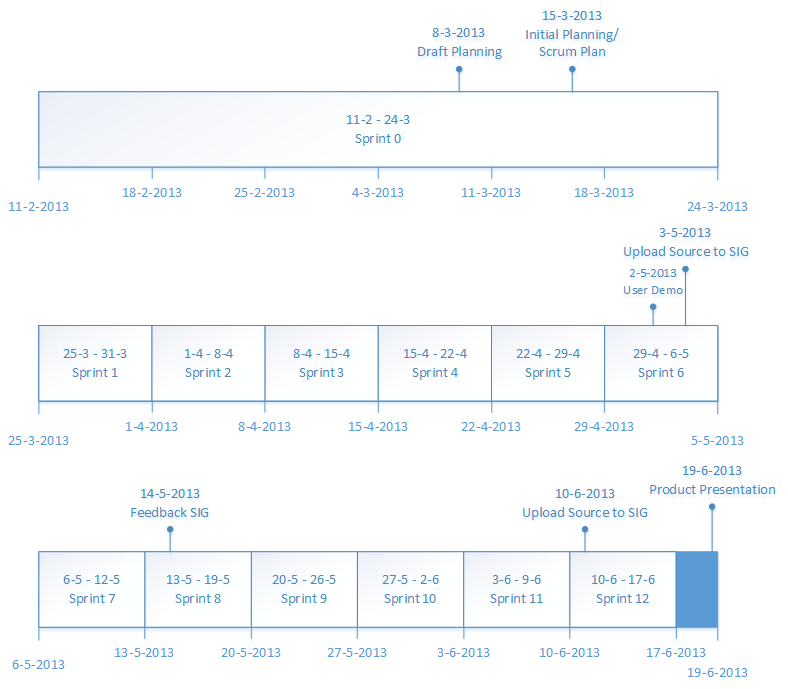
\includegraphics[scale=1]{Roadmap.png}}
			\caption{Roadmap}
			\label{fig: Roadmap}
			\end{figure}	
			\subsubsection*{Sprint 0}
				\textbf{Q3/W4 Draft planning:}\\ The product and domain are researched, the product vision and high-level product backlog are devised with initial list of user stories composed. The user stories can be found under the product backlog.\\
				\textbf{Q3/W5 Initial planning:}\\ The user story list is fine-tuned and tasks devised for the first sprints.\\
				The user stories can be found under the product backlog. After this sprint all data models for should be present.\\		
				\textbf{Q3/W6}\\
				Toolchain needed to develop the code is set up. Basic module and cell classes are made and properly tested.
			\subsubsection*{Sprint 1 (Q3/W7)}
				The properties of the modules are not static but can be changed. Start working on integration tests.
			\subsubsection*{Sprint 2 (Q3/W8)}
				The cell environment can be changed by adding substrates. Modules can react on these substrates.
			\subsubsection*{Sprint 3 (Q3/W9)}
				A basic visualisation of the model data is present. This consists of at least one graph per module that indicates the concentration over time. A set of static modules is available for model composition.
			\subsubsection*{Sprint 4 (Q3/W10) Demo product}
				The product should be usable, stable and completed in terms of the items that are considered MUST. This means that the first 4 items from the High-Level Product backlog are incorporated in this demo. The demo consists of a series of acceptance tests devised in sprint 4.
			\subsubsection*{Sprint 5 (Q4/W1)}
				The output can be exported as a document (HTML/PDF/Excel). Initial rigorous acceptance tests, as the next sprint as a product demo. The models created can now be saved and loaded. Feedback on module constraints is visible
			\subsubsection*{Sprint 6 (Q4/W2)}
				Feedback on errors and optimisation is now visible in the application.
			\subsubsection*{Sprint 7 (Q4/W3)}
				Fixing failing unit/functional tests and conducting acceptance tests.\\
			\subsubsection*{Sprint 8 (Q4/W4)}
				The product is internationalised.
			\subsubsection*{Sprint 9 (Q4/W5)}
				Bug-fixes, acceptance tests and final review of code. Prepare for SIG review.
			\subsubsection*{Sprint 10 (Q4/W6)}
				The product should be usable, stable and completed in terms of the items that are considered MUST (First four in the high level product backlog) and SHOULD (Item 5 and 6 in the high level product backlog).
			\subsubsection*{Sprint 11 (Q4/W7)}
			\subsubsection*{Sprint 12 (Q4/W8) Final product}

	\clearpage
	\section{Product backlog}
		The product backlog is a list of requirements that must be met for the product. The priority of each story is defined by its position in the backlog. The higher on the backlog, the more important the item is.\\
		\\
		\textbf{A user can create a cell consisting of modules}. \\
		\indent
			\textit{Note: modules are processes like transporters bringing in substrates or ejecting products\\
		\indent
			Modules can be selected from a list and placed in the cell.\\
		\indent
			Estimate: 6 hours} \\
		\textbf{A user can see the output of the simulation. }\\
		\indent
			\textit{Note: a visual representation of the reactions with a module in the form of graphs. \\
		\indent
			Estimate: 4 hours} \\\
		\textbf{A user can change the module properties such as the reaction speed.} \\
		\indent
			\emph{Estimate: 8 hours} \\
		\textbf{A user can add substrates to the cell.} \\
		\indent
			\emph{Estimate: 4 hours} \\
		\textbf{A user can generate an HTML report of the simulation. This contains parameter values and concentration graphs from all the modules.} \\
		\indent
			\emph{ Estimate: 12 hours} \\
		\textbf{A user can generate PDF and Excel reports, equivalent to the HTML report.} \\
		\indent
			\emph{Estimate: 4 hours} \\
		\textbf{A user can save and load a model.} \\
		\indent
			\emph{Estimate: 8 hours} \\
		\textbf{A user gets feedback on his model, such as missing modules, errors, constraints and possible optimisations if possible (maximising the yield, for example).} \\
		\indent
			\emph{Estimate: 12 hours} \\
		\textbf{A user can change the equations representing the different reactions.} \\
		\indent
			\emph{Estimate: 4 hours} \\
		\textbf{A user can change the language.} \\
		\indent
			\emph{Estimate: 8 hours} \\
		\textbf{A user can select parameter sets for modules based on existing DNA sequences known to generate a module with such reaction parameters.} \\
		\textbf{A user can view a phenotype of a model on his/her phone.} \\
		\textbf{A user can edit a cell model on his phone.} \\
		\textbf{A user can create new modules on his phone.} \\
		\textbf{A user can add modules to an existing cell model.} \\

	\clearpage
	\section{Definition of done}
		Defining when the following are done is important to keep the flow in the project and make sure the product is deliverable. \\
		\\
		\textbf{Task:} If the description is fulfilled and this can be verified with a \emph{user} and/or an \emph{integration} test. {\scriptsize This is important because features have to be complete, else there will be unfinished code in the system which will cause instability.}\\
		\textbf{User Story:} If the story is fulfilled and this can be tested with an \emph{acceptance test}.  {\scriptsize This is important because the user stories are the basis to defining the functions the system must provide.}\\
		\textbf{Sprint:} Sunday 23:59. { \scriptsize This is important because it limits the amount of work done during a sprint.}\\
		(version of a) \textbf{Product/Release:} If the product can be shipped to the \emph{stakeholder}. { \scriptsize This is important because this is what the stakeholder gets to see. It can be shipped when all features which are considered a MUST and SHOULD are implemented, see the high-level product backlog and roadmap} \\
		\textbf{Project:} Never or when the \emph{stakeholder} decides (\emph{June 14$^{th}$}).

	\section{Glossary}
		\textbf{Backlog Item}\\
		A unit of work small enough to be completed by a team in one sprint iteration. Backlog items are decomposed into one or more tasks. \\
		\\
		\textbf{Demo}\\
		A session of testing with one or more stakeholders, where they evaluate the product. \\
		\\
		\textbf{Release} \\
		The transition of an increment of potentially shippable product from the development team into routine use by customers. Releases typically happen when one or more sprints has resulted in the product having enough value to outweigh the cost to deploy it. \\
		\\
		\textbf{Sprint} \\
		A one week period during which the team selects features of a product from the product backlog and finishes it by the end of the week. \\
		\\
		\textbf{Task} \\
		A sprint task (or task) is a unit of work small enough to be completed by a team member in a matter of hours. \\
		\\
		\textbf{User Story} \\
		One or more sentences in the everyday or business language of the end user that capture which action a user should perform to accomplish a specific goal with the product. The basis for defining the functions a business system must provide.
\end{document}

